\documentclass[letterpaper,10pt]{article}

\usepackage{geometry}
\usepackage{glossaries}
\usepackage{hyperref}
\usepackage[pdftex]{graphicx}
\usepackage{tikz}
\usepackage{wrapfig}
\geometry{textheight=8.5in, textwidth=6in}
\newenvironment{bottompar}{\par\vspace*{\fill}}{\clearpage}

\makeglossaries
\newglossaryentry{payload}{
	name=payload,
	description={A subsection of a rocket that is not essential to the rocket's 
		operation. A payload is placed in a can, mounted on a standard base plate. 
		A payload completes some specific task.}
}

\newglossaryentry{can}{
	name=can,
	description={A can is a segment of the rocket in which payloads can be 
		placed. A can constitutes a standard length of rocket, defined by the 
		RockSat-X program.}
}

\newglossaryentry{Arm Assembly}{
	name={Arm Assembly},
	description={The Hephaestus Arm Assembly includes the arm, the rotating arm
		base, the camera, and base. It is the portion of the payload that is 
		extended during Science mode.}
}

\newglossaryentry{api}{
	name=API,
	description={Application Programming Interface. The set of functions and 
		classes that a given library exposes for other programs to make use of its
		provided functionality.}
}

\newglossaryentry{ascii}{
	name=ASCII,
	description={American Standard Code for Information Interchange. Each 
		alphabetic, numeric, or special character is represented with a 7-bit 
		binary number. 128 possible characters are defined.}
}

\newglossaryentry{port}{
	name=port,
	description={To transfer software from one system or machine to another.}
}

\newglossaryentry{ter}{
	name=TE-R,
	description={The TE-R line is a redundant electrical input to the system
		that enables at a predetermined time during flight.}
}

\newglossaryentry{te1}{
	name=TE-1,
	description={The TE-1 line is an electrical input to the system that 
		enables at a predetermined time during flight.}
}

\newglossaryentry{replay}{
	name=replay,
	description={To replay a dataset is to reproduce preexisting data in a manner that
		simulates how it was generated, e.g. output the data in the same timeline that each
		data point was generated.}
}

\newglossaryentry{plot}{
	name=plot,
	description={An interactive window generated by the Python library matplotlib to
		display some dataset on an x and y axis.}
}

\newglossaryentry{apogee}{
	name=apogee,
	description={The point at which the rocket has finished its ascent and payloads
		are allowed to deploy.}
}

\newglossaryentry{matplotlib}{
	name=matplotlib,
	description={A Python library for drawing and manipulating graphs.}
}

\newglossaryentry{binstring}{
	name=binary string,
	description={An ordered sequence of 1's and 0's.}
}

\newglossaryentry{deployable}{
	name=deployable,
	description={Any portion of the payload that is expanded from its original 
		configuration once in a space-like environment.}
}

\newglossaryentry{npm}{
	name=npm,
	description={npm is a package manager for NodeJS, a javascript library. It
		is used to install various `npm' packages for NodeJS servers.}
}

\newglossaryentry{cspace}{
	name=configuration space,
	description={The Configuration Space (or C-Space) is a 4 dimensional space with
		a mapping to 3D real space that is used to represent the possible 
		configurations of the arm's motors.}
% Removed the following lines because the definition is not the appropriate
% place to explain implementation details.
% The C-Space is stored in a 4D array of 
%characters. Possible valid configurations are marked as such in the C-Space and 
%this data is used to plot the arm's path.}
}

\newglossaryentry{dof}{
	name=degree-of-freedom,
	description={The directions in which independent motion can occur. In the case of the Hephaestus arm, there are four degrees of freedom.}
}

\newglossaryentry{obc}{
	name={on-board computer},
	description={The microcontroller responsible for the control and experiment systems on the payload.}
}

\newglossaryentry{microgravity}{
	name=microgravity,
	description={An environment where the effect of gravity is significantly less than earth's.}
}

\newglossaryentry{eeprom}{
	name=EEPROM,
	description={Electrically erasable programmable read-only memory. A type of	
		persistent storage for small amounts of data.}
}

\newacronym{psu}{PSU}{Portland State University}
\newacronym{psas}{PSAS}{Portland State Aerospace Society}
\newacronym{gui}{GUI}{Graphical User Interface}
\newacronym{wff}{WFF}{Wallops Flight Facility}
\newacronym{osu}{OSU}{Oregon State University}
\newacronym{OBC}{OBC}{On-Board Computer}
\newacronym{aiaa}{AIAA}{American Institute of Aeronautics and Astronautics}

\title{Technical Review And Implementation Plan For RockSat-X Payload - Hephaestus}
\author{Helena~Bales, Amber~Horvath, and Michael~Humphrey\\ \\ CS461 - Fall 2016}

\parindent = 0.0 in
\parskip = 0.1 in

\begin{document}
\maketitle

\begin{abstract}
The \gls{OSU} RockSat-X team shall be name Hephaestus.
The possible methods for implementing our project requirements shall be outlined in this document.
The mission requires that the payload, an autonomous robotic arm, perform a series of motions to locate predetermined targets.
The hardware shall be capable of performing the motions to reach the targets.
The software shall determine the targets and send the commands to the hardware to execute the motion.
The combination of the hardware controlled by the software shall demonstrate Hephaestus's ability to construct small parts on orbit.
This document will focus on the implementation of the software, but shall include necessary project context including hardware.
\end{abstract}

\begin{bottompar}
Approved By
\_\_\_\_\_\_\_\_\_\_\_\_\_\_\_\_\_\_\_\_\_\_\_\_\_\_\_\_\_\_\_\_\_\_\_\_\_\_\_\_\_\_\_\_\_\_\_\_\_\_\_\_\_\_\_\_\_\_\_\_\_\_\_
Date \_\_\_\_\_\_\_\_\_\_\_\_\_\_\_\_\_\_\_\_\_\_\_\_\_\_\_\_ \\


Approved By
\_\_\_\_\_\_\_\_\_\_\_\_\_\_\_\_\_\_\_\_\_\_\_\_\_\_\_\_\_\_\_\_\_\_\_\_\_\_\_\_\_\_\_\_\_\_\_\_\_\_\_\_\_\_\_\_\_\_\_\_\_\_\_
Date \_\_\_\_\_\_\_\_\_\_\_\_\_\_\_\_\_\_\_\_\_\_\_\_\_\_\_\_ \\


Approved By
\_\_\_\_\_\_\_\_\_\_\_\_\_\_\_\_\_\_\_\_\_\_\_\_\_\_\_\_\_\_\_\_\_\_\_\_\_\_\_\_\_\_\_\_\_\_\_\_\_\_\_\_\_\_\_\_\_\_\_\_\_\_\_
Date \_\_\_\_\_\_\_\_\_\_\_\_\_\_\_\_\_\_\_\_\_\_\_\_\_\_\_\_ \\


Approved By
\_\_\_\_\_\_\_\_\_\_\_\_\_\_\_\_\_\_\_\_\_\_\_\_\_\_\_\_\_\_\_\_\_\_\_\_\_\_\_\_\_\_\_\_\_\_\_\_\_\_\_\_\_\_\_\_\_\_\_\_\_\_\_
Date \_\_\_\_\_\_\_\_\_\_\_\_\_\_\_\_\_\_\_\_\_\_\_\_\_\_\_\_ \\
\end{bottompar}

\clearpage
\tableofcontents
\clearpage

\section{Introduction}
\subsection{Document Overview}
This is the Technical Review And Implementation Plan for the Hephaestus project.
This document shall investigate possible methods of implementing our project software requirements.
The nine general requirements investigated below were identified as project requirements in our Requirements document.
This document will focus on the "how" of our requirements implementation.
\subsection{Role Breakdown}
Each CS Senior Design team member shall be responsible for insuring the completion of the three items
from the requirements document that are assigned to them below.
\subsubsection{Helena Bales}
\begin{enumerate}
\item{Target Generation}
\item{Arm Movement}
\item{Arm Position Tracking}
\end{enumerate}
\subsubsection{Amber Horvath}
\begin{enumerate}
\item{Emergency Payload Expulsion}
\item{Program Modes of Operation}
\item{Target Success Sensors}
\end{enumerate}
\subsubsection{Michael Humphrey}
\begin{enumerate}
\item{Telemetry}
\item{Video Camera}
\item{Data Visualization and Processing}
\end{enumerate}

\section{Technologies}
\subsection{Target Generation}
\subsubsection{Requirement Overview}
The software shall generate points to be used in testing the Hephaestus arm.
The points will constitute the total test of the arm, and should therefore include points
representative of standard and edge cases.
These points shall be used as targets for the arm body.
\subsubsection{Proposed Solutions}
\begin{enumerate}
\item{
\textbf{The points shall be generated in 3-D polar form}, including an angle from normal, a radius, 
and a height. 
The angle shall be in the range of 0 and 359 degrees.
An angle of zero degrees shall be in the direction of payload deployment.
The radius shall be the distance from the arm's attachment to the base to the generated point.
The height of the point, for the purpose of target generation, shall be constant.
However the points will always be stored in a triple of angle from normal (\(\theta\)), radius (\(r\)), and height (\(h\)).
}
\item{
\textbf{The points shall be generated in 3-D Cartesian form}, including \(x\) position to the right 
or left of the \(y-axis\), the \(y\) position above or below the \(x-axis\), and the height, \(h\), 
above the \(xy-plane\).
Let the \(y-axis\) be the direction that the payload deploys from the can.
Let the \(x-axis\) be the perpendicular to the \(y-axis\) at the point where the arm is mounted 
to the rotating plate. 
Let \(h\) be the height above the \(xy-plane\), where the arm is attached to the rotating plate.
}
\item{
\textbf{The points shall be generated in 2-D Polar coordinates}, where the implementation is the 
same as described in the 3-D Polar coordinate section, with the exception of \(h\).
In this case, there shall be no \(h\).
The position can be represented in 2-D Polar coordinates on the plane of the base plate.
For the purpose of compatability with the position of the arm, the height could be assumed to be 0.
}
\end{enumerate}

\subsection{Arm Movement}
\subsubsection{Requirement Overview}
The software shall control the movement of the arm body assembly. 
The position of the tip of the arm shall be tracked in the coordinate notation described in section 2.2 above.
The software shall rotate the arm body assembly in a full 360 degrees.
The software shall additionally control the movement the height of the arm body assembly.
The arm should descend and touch the baseplate of the payload at any rotation.

TODO ADD MORE
\subsubsection{Proposed Solutions}

\subsection{Arm Position Tracking}
\subsubsection{Requirement Overview}
The position of the arm shall be tracked using the same coordinate system described in the Target Generation requirement.
The position of the arm shall be calculated using the known start position and the rotation of the motors.
The starting position shall be known due to a calibration point that will allow for a reset at any time.
Resetting in this way will allow for flexibility between resetting for maximum operation time with only tolerably small error defined by the Non Functional Requirements.
\subsubsection{Proposed Solutions}

\subsection{Tech 4}
\subsubsection{Requirement Overview}
\subsubsection{Proposed Solutions}
\subsection{Tech 5}
\subsubsection{Requirement Overview}
\subsubsection{Proposed Solutions}
\subsection{Tech 6}
\subsubsection{Requirement Overview}
\subsubsection{Proposed Solutions}
\subsection{Telemetry}
\subsubsection{Requirement Overview}
\subsubsection{Proposed Solutions}
The three options being considered for transmitting telemetry are
\begin{enumerate}
\item{A custom-built solution for our own needs}
\item{Open MCT developed by NASA for space-specific missions}
\item{TODO} 
\end{enumerate}

\subsection{Video Handling}
\subsubsection{Requirement Overview}
\subsubsection{Proposed Solutions}

\subsection{Data Visualization}
\subsubsection{Requirement Overview}
\subsubsection{Proposed Solutions}

\section{Conclusion}
\section{Glossary}

\section{Appendix}
\subsection{Mission Patch}
\includegraphics[width=\textwidth]{logo}
\begin{center}
\textbf{Figure 1: Mission Logo [1]}
\end{center}

\subsection{Project Overview}
The Hephaestus project is a Capstone Senior Design project for Oregon State University's 2016/2017 Senior Design class (CS461-CS463).
The CS senior design project is one part of the overall Hephaestus project.
In addition to the CS team, there is one team of Electrical Engineers and two teams of Mechanical Engineers working on this project through other senior design classes.
The Hephaestus payload is a rocketry payload developed as part of the 2016/2017 RockSat-X program.
The RockSat-X program is a year long program where groups of students develop rocketry payloads with the help of the Colorado Space Grant Consortium and Wallops Flight Facility.
The term "rocketry payload" refers to an experiment inside a section of the rocket.
Each section of the rocket is called a can, and is a standard space that we can fill with an experiment.
The Hephaestus payload shall take up half a can and shall be mounted on a standard base plate provided by Wallops.
We, as the Hephaestus team, will create the hardware and software for the payload, then integrate it into the rocket before launch.

\subsubsection{Project Phases}
The project shall include several phases. The first is the design phase.
The design phase shall last all of Fall 2016 term at OSU.
In the design phase, we shall design the robotics, electronics, materials, and software.
The design phase shall include presentations to the RockSat-X program, where there will review our designs.
Following the design phase will be the implementation phase.
In the implementation phase we shall last through June 2017.
This phase shall include testing of the payload.
We will perform testing both at OSU and at Wallops.
At OSU we will be testing the payload functionality.
At Wallops, we will be testing the structural integrity of the payload, as well as its resistance to vibrations, heat, and cold.
Following the implementation phase will be the integration phase.
This phase will occur at Wallops in July.
This is the point at which our base plate will be integrated into the rocket as a whole, along with the other participating teams.
The final phase will be launch. Launch will occur in Summer of 2017.
The rocket shall be launched from Wallops Flight Facility.
During the flight we shall send telemetry to the ground station at Wallops.
The payload shall perform the experiment once it reaches appogee.
The payload will hopefully be recovered post-flight.

\subsection{Software State Diagram}
\begin{center}
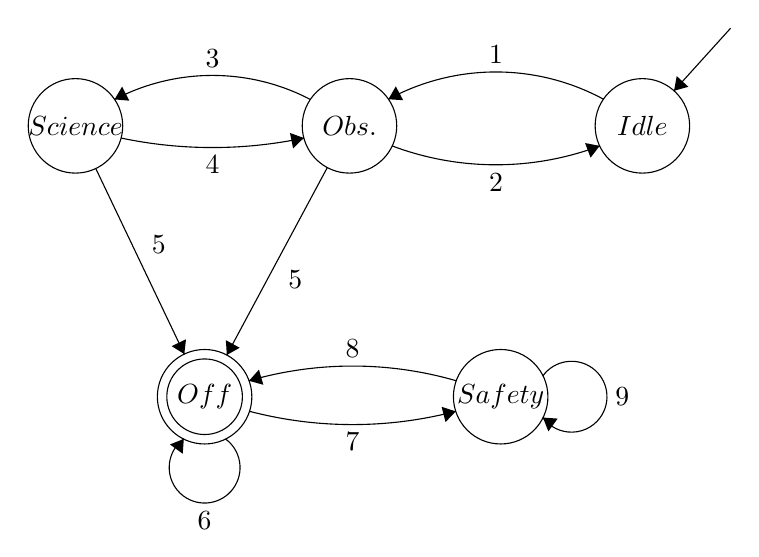
\begin{tikzpicture}[scale=0.2]
\tikzstyle{every node}+=[inner sep=0pt]
\draw [black] (24.2,-19.2) circle (3);
\draw (24.2,-19.2) node {$Obs.$};
\draw [black] (42.8,-19.2) circle (3);
\draw (42.8,-19.2) node {$Idle$};
\draw [black] (6.8,-19.2) circle (3);
\draw (6.8,-19.2) node {$Science$};
\draw [black] (15,-36.4) circle (3);
\draw (15,-36.4) node {$Off$};
\draw [black] (15,-36.4) circle (2.4);
\draw [black] (33.8,-36.4) circle (3);
\draw (33.8,-36.4) node {$Safety$};
\draw [black] (48.4,-13) -- (44.81,-16.97);
\fill [black] (44.81,-16.97) -- (45.72,-16.72) -- (44.98,-16.04);
\draw [black] (26.67,-17.507) arc (118.43354:61.56646:14.344);
\fill [black] (26.67,-17.51) -- (27.61,-17.57) -- (27.14,-16.69);
\draw (33.5,-15.28) node [above] {$1$};
\draw [black] (40.088,-20.475) arc (-69.41442:-110.58558:18.736);
\fill [black] (40.09,-20.47) -- (39.16,-20.29) -- (39.51,-21.22);
\draw (33.5,-22.17) node [below] {$2$};
\draw [black] (9.281,-17.525) arc (117.61533:62.38467:13.416);
\fill [black] (9.28,-17.52) -- (10.22,-17.6) -- (9.76,-16.71);
\draw (15.5,-15.5) node [above] {$3$};
\draw [black] (21.303,-19.973) arc (-78.10445:-101.89555:28.152);
\fill [black] (21.3,-19.97) -- (20.42,-19.65) -- (20.62,-20.63);
\draw (15.5,-21.08) node [below] {$4$};
\draw [black] (8.09,-21.91) -- (13.71,-33.69);
\fill [black] (13.71,-33.69) -- (13.82,-32.75) -- (12.91,-33.19);
\draw (11.61,-26.74) node [right] {$5$};
\draw [black] (16.323,-39.08) arc (54:-234:2.25);
\draw (15,-43.65) node [below] {$6$};
\fill [black] (13.68,-39.08) -- (12.8,-39.43) -- (13.61,-40.02);
\draw [black] (22.79,-21.85) -- (16.41,-33.75);
\fill [black] (16.41,-33.75) -- (17.23,-33.29) -- (16.35,-32.81);
\draw (20.28,-28.97) node [right] {$5$};
\draw [black] (30.948,-37.326) arc (-75.33467:-104.66533:25.865);
\fill [black] (30.95,-37.33) -- (30.05,-37.04) -- (30.3,-38.01);
\draw (24.4,-38.67) node [below] {$7$};
\draw [black] (17.821,-35.385) arc (106.14932:73.85068:23.653);
\fill [black] (17.82,-35.39) -- (18.73,-35.64) -- (18.45,-34.68);
\draw (24.4,-33.95) node [above] {$8$};
\draw [black] (36.48,-35.077) arc (144:-144:2.25);
\draw (41.05,-36.4) node [right] {$9$};
\fill [black] (36.48,-37.72) -- (36.83,-38.6) -- (37.42,-37.79);
\end{tikzpicture}
\end{center}
\begin{center}
Diagram of software states of operation and transition between states [2].

Transitions between states occur as numbered:

\begin{enumerate}
\item{\textbf{Appogee is reached.} The software shall activate when the power line goes to high at 28V. Observation mode shall be triggered when the OBC turns on.}
\item{\textbf{Error: Return to Idle.} If an error is encountered in entering Observation mode, the software shall fallback to Idle mode and retry. An error may occur if the payload fails to deploy correctly or if the camera fails to turn on.}
\item{\textbf{Payload Assembly and Camera have been deployed.} The software shall enter science mode once the payload assembly and arm have deployed and the camera has performed an observation sweep.}
\item{\textbf{Error: Return to Observation} The software shall return to observation mode if any error occurs in Science mode. An error may occur in Science mode if the arm fails to operate correctly and must return to default position. An error may also occur if the camera stops working.}
\item{\textbf{Timer switches to end appogee period.} Once the time period for observation has ended, the timer line will go to low and trigger to Shutdown state. This state can be reached from either Observation or Science mode.}
\item{\textbf{Accept: Shutdown correctly} If Shutdown occurs correctly, the arm should be closed, the Arm Assembly Body should be retracted, and the OBC should be powered off.}
\item{\textbf{Error: Shutdown not completed successfully.} If an error occurs in the shutdown sequence, the software shall enter Safety mode.}
\item{\textbf{Payload is Shutdown correctly.} If the payload is Shutdown through Safety mode, shutdown can be completed. In Safety mode the payload was either shut down correctly, retracted fully into the can with the arm open, or the arm was expelled safely from the rocket.}
\item{\textbf{Error: Payload is still deployed.} The software shall remain in Safety mode until the payload is either retracted correctly, retracted fully with the arm in the open position, or ejected safely from the rocket. Safety mode shall first try to correctly retract the arm, then retract with the arm open, then repeat attempting ejection until the payload is ejected.}
\end{enumerate}
\end{center}

\subsection{Model of Payload Hardware}
\subsection{Payload Wiring Diagram}
\subsection{References}
[1] TODO Who made the Logo for us?
[2] H. Bales and M. Humphrey, "Diagram of Software Modes of Operation," 2016. [Online]. Available: Hephaestus Requirements Document.



\end{document}
